% !TeX TS-program = xelatex
% !BIB TS-program = bibtex

% Full instructions available at:
% https://github.com/pcafrica/focus-beamertheme


\documentclass{beamer}
\usepackage[yyyymmdd]{datetime}
\usepackage{tikz}
\usetikzlibrary{quantikz2}
\usepackage{amsmath}
\usepackage{xfrac}
\usepackage{mathdots}
\usepackage{nccmath}
\usetheme{focus}


\definecolor{main}{RGB}{55, 135, 177}
\definecolor{text}{RGB}{60, 60, 80}
\definecolor{background}{RGB}{255, 255, 255}

\setmathfont{Latin Modern Math}[range={frak,\bigcap,\bigcup}]
\newif\ifplacelogo % create a new conditional
\placelogotrue % set it to true


\newcommand{\foralll}[2]{\overset{{#2}}{\underset{{#1}}{\Large \forall}}}
\newcommand{\existss}[2]{\overset{{#2}}{\underset{{#1}}{\Large \exists}}}

\setbeamercovered{transparent}

\title{Into the Quantum Realm:\\ On the Collapsible Polynomial Hierarchy for Promise Problems}
\subtitle{Advance Algorithm Course}
\author{Abolfazl Ghorbani\texorpdfstring{\\}{,} Asha Soroushpoor}
% \titlegraphic{
\includegraphics[scale=1.25]{focus-logo.pdf}}
\titlegraphic{
\includegraphics[scale=.21]{images/tu-logo-hckd2.png}}
\logo{\ifplacelogo
\includegraphics[height=1cm]{images/tu-logo-hckd2.png}\fi}
\institute{University of Tehran}
\date{\today}



% Footline info is printed only if [numbering=fullbar].
%\footlineinfo{Custom footline text}

\begin{document}
    \placelogofalse
\begin{frame}
    \maketitle
\end{frame}

\begin{frame}
    \frametitle{Table of Contents}
    \tableofcontents
\end{frame}
\placelogotrue
    
    
    % Use starred version (e.g. \section*{Section name})
    % to disable (sub)section page.
    \section{The Polynomial-time Hierarchy}
    \subsection{Basic definitions and properties}
        \begin{frame}{Definitions}
            \begin{block}{Definition: $\Sigma_k^P$}
                $ \Sigma_0^P := P$\\
                For $k\geq 1:$ \\
                $L \in \Sigma_k^P \iff $ there are polynomials $p_1, p_2,..., p_k$ and a polynomial-time predicate $F$ s.t.:
                $$x \in L \leftrightarrow 
                    \existss{y_1 \in S_1\text{ }}{}
                    \foralll{y_2 \in S_2\text{ }}{}
                    \exists ...\underset{y_k \in S_k}{Q} F(x,y_1,...,y_k)$$
                where $S_i := \{0,1\}^{p_i(|x|)}$  
            \end{block}
        \end{frame}
        \begin{frame}{Definitions}
            \begin{block}{Definition: $\Pi_k^P$}
                $ \Pi_0^P := P$\\
                For $k\geq 1:$ \\
                $L \in \Pi_k^P \iff $ there are polynomials $p_1, p_2,..., p_k$ and a polynomial-time predicate $F$ s.t.:
                $$x \in L \leftrightarrow 
                    \foralll{y_1 \in S_1\text{ }}{}
                    \existss{y_2 \in S_2\text{ }}{}
                    \forall ...\underset{y_k \in S_k}{Q} F(x,y_1,...,y_k)$$
                where $S_i := \{0,1\}^{p_i(|x|)}$  
            \end{block}
        \end{frame}

        
        \begin{frame}{Definitions}
            \begin{block}{Definition: The Polynomial-time Hierarchy $PH$}
            $PH := \bigcup_{i \in \mathbb{N}} \Sigma_i^P \cup \Pi_i^P $
            \end{block}
        \end{frame}
    
        \begin{frame}{Structural Properties}  
            for all $i\in \mathbb{N}$: 
            \begin{enumerate}
                \item $\Pi_i^P = co\Sigma_i^P $
                \pause
                \item $\Sigma_i^P \subseteq \Sigma_{i+1}^P \cap \Pi_{i+1}^P$
                \item $\Pi_i^P \subseteq \Sigma_{i+1}^P \cap \Pi_{i+1}^P$
                \pause
                \item (?)$\Sigma_i^P \subset \Sigma_{i+1}^P$
            \end{enumerate}
        \end{frame}

        \begin{frame}{Equivalent definition}
            \begin{block}{lemma}
                For $i\geq 1, L \in  \Sigma_{i+1}^P \iff $there is a polynomial $p$ and $A \in \Pi_i^P$:
                $$x \in L \leftrightarrow \existss{y\in \{0,1\}^{p(|x|)}}{} <x,y> \in A$$
            \end{block}
            \pause
            \begin{block}{Proof}
                $<x,y> \in A \leftrightarrow \foralll{y_1 \in S_1\text{ }}{}
                    \existss{y_2 \in S_2\text{ }}{}
                    \forall ...\underset{y_k \in S_k}{Q} F(<x,y>,y_1,...,y_k)$\\
                for some polynomial F and $S_i := \{0,1\}^{p(|x|)_i}$ for polynomials $p_1,p_2,..., p_k$. Putting this in the equation gives us the desired result.
            \end{block}
        \end{frame}

        \begin{frame}{Collapsibility}
            \begin{block}{lemma}
                For $i\geq 1, L \in  \Pi_{i+1}^P \iff $there is a polynomial $p$ and $A \in \Sigma_i^P$:
                $$x \in L \leftrightarrow \foralll{y\in \{0,1\}^{p(|x|)}}{} <x,y> \in A$$
            \end{block}
            \pause
            \begin{block}{Theorem: PH is collapsible}            
                $i \geq 1 $ \& $ \Pi_i^P = \Sigma_i^P \to PH = \Sigma_i^P$
            \end{block}
        \end{frame}

        \begin{frame}{Collapsibility}
            \begin{proof}
                \small{
                It suffices to show that 
                $i\geq1 \text{ $\&$ } \Sigma_k^P = \Pi_k^P 
                \to \Sigma_k^P = \Sigma_{k+1}^P$:\\
                $L \in \Sigma_{k+1}^P \iff$ there is a polynomial $p$ and $A \in \Pi_i^P$:
                $$x \in L \leftrightarrow \existss{|y|=p(|x|)}{} <x,y> \in A$$
                $\iff$ there are $A \in \Sigma_i^P$ and $p$:
                 $...$\\
                $\iff$ there are $p,p'$ and $B \in \Pi_{i-1}^P$:
                $$x \in L \leftrightarrow \existss{|y|=p(|x|)}{} \existss{|y'|=p'(|x|)}{} <x,y,y'> \in B$$
                $\iff$ there are $p'' = p+p'$ and $B \in \Pi_{i-1}^P$:
                $$x \in L \leftrightarrow \existss{|y''|=p"(|x|)}{} <x,y''> \in B$$
                $\iff L \in \Sigma_k^P$.
                }
            \end{proof}
        \end{frame}
            

        \begin{frame}{Scheme of the Polynomial-time hierarchy}            
            \begin{figure}
                \centering
                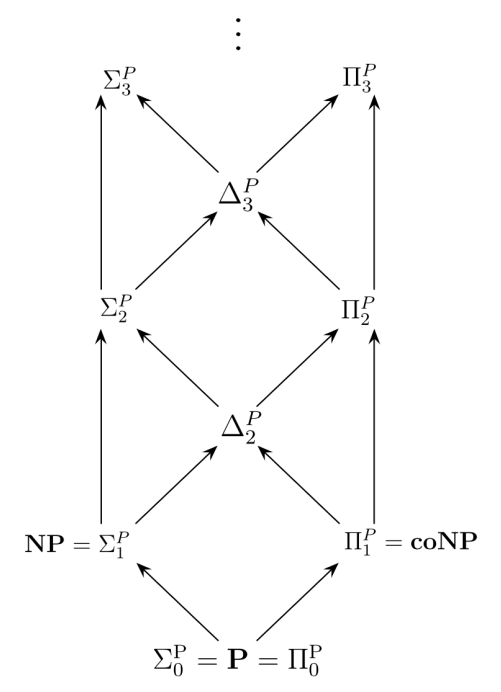
\includegraphics[scale=.4]{images/PH.png}
                \caption{The Polynomial-time Hierarchy.}
                \label{fig:The Polynomial-time Hierarchy}
            \end{figure}
        \end{frame}

    \subsection{Relationships to other  complexity classes}
        \begin{frame}{Relationships to other complexity classes}  
            \begin{block}{Review: NP}
                $L \in NP \iff $ there is a polynomial $p$ and a Polynomial-time predicate $F$ s.t.:
                $$x \in L \iff \existss{y \in O(p(|x|))}{} F(x,y)$$
            \end{block}
        \end{frame}
        \begin{frame}{Relationships to other  complexity classes}
            \begin{block}{Lemma}
                $NP = \Sigma_1^P$
            \end{block}
            \begin{block}{Proof}
                \begin{enumerate}
                    \item $\existss{p}{}  y \in O(p(|x|) \iff \existss{p'}{}  y\leq  \, p'(x)$
                    \item  for one direction use padding to fix the length of y
                    \item for the other direction check the length of y in algorithm
                \end{enumerate}                
            \end{block}
        \end{frame}
        
        \begin{frame}{Relationships to other  complexity classes} 
            \begin{block}{Definition: BPP}
                $L \in BPP \iff $ there is a polynomial $p$ and a polynomial-time randomized algorithm (predicate) $F$ s.t.:
                $$x \in L \implies \underset{r\in \{0,1\}^{p(|x|)}}{Pr}(F(x,r)) \geq 2/3$$
                $$x \notin L \implies \underset{r\in \{0,1\}^{p(|x|)}}{Pr}\ (F(x,r)) \leq 1/3$$
            \end{block}
            \begin{table}
                \centering
                \begin{tabular}{rcc}
                     & $F(x,r)$ & $\neg F(x,r)$ \\\hline
                    $x \in L$ & \(\geq 2/3\) & \(\leq 1/3\) \\
                    $x \notin L$ & \(\leq 1/3\) & \(\geq 2/3\) \\
                \end{tabular}
                \caption{$\underset{r\in \{0,1\}^{p(|x|)}}{Pr}\ (F(x,r))$}
                \label{BPP DEF}
            \end{table}
        \end{frame}
        
        %\begin{frame}{Relationships to other complexity classes}
        %    \begin{lemma}
        %        If $L \in BPP$, then there is a polynomial time algorithm %$A$ such that: $$\underset{r\in \{0,1\}^m} {P}\ (A(x,r) = %right\text{ }answer) \geq 1-\frac{1}{3m}$$
        %        where $m = |x|^k$ for some $k$.
        %    \end{lemma}
        %\end{frame}
        
        %\begin{frame}{Relationships to other complexity classes}
        %    \begin{alertblock}{proof}
        %        There is a polynomial time algorithm A; $\underset{r'\in \%{0,1\}^m} {P}\ (A(x,r') = right\text{ }answer) \geq \frac{2}{3m}$
        %        Design F(x,r):= which takes     
        %    \end{alertblock}
        %\end{frame}

        \begin{frame}{Relationships to other complexity classes}
            \begin{block}{lemma}
                $BPP$ is closed under complement.
            \end{block}
            
            \begin{block}{Fact}
                $BPP \subseteq \Sigma_2$
            \end{block}
        \end{frame}
                
        \begin{frame}{Relationships to other complexity classes}
            \begin{block}{Sipser–Lautemann theorem}
                $BPP \subseteq \Sigma_2^P \cap \Pi_2^P$
            \end{block}
        \end{frame}
        
        \begin{frame}{Relationships to other  complexity classes}
            \begin{block}{Theorem}
                $PH \subseteq PSPACE$
            \end{block}
        \end{frame}

        \begin{frame}{Relationships to other  complexity classes}
            \begin{block}{Proof}
                It is sufficient to show that for any $i$ if $\Pi_i \in PSPACE$ then $\Sigma_{i+1} \in PSPACE$:\\
                Suppose $L \in \Sigma_{i+1}$ then there is a polynomial $p$ and $A \in \Pi_i^P$:
                $$x \in L \leftrightarrow \existss{y\in \{0,1\}^{p(|x|)}}{} <x,y> \in A$$
                $A$ is decidable in $PSPACE$ by hypothesis, thus $\existss{y\in \{0,1\}^{p(|x|)}}{} <x,y> \in A$ is decidable in $PSPACE$ using an odometer.
            \end{block}
        \end{frame}

        \begin{frame}{Relationships to other  complexity classes}
            \begin{block}{Lemma}
                For all $i$: $\Sigma_i^P$  is closed under $\leq_p$
            \end{block}
            \pause
            \begin{block}{Proof}
                $A \leq_p B \iff$ there is a polynomial algorithm $R$:
                    $$x\in A \iff R(x) \in B$$
                Now suppose $B \in \Sigma_i^P$ then:
                $$x \in A \leftrightarrow 
                    \existss{y_1 \in S_1\text{ }}{}
                    \foralll{y_2 \in S_2\text{ }}{}
                    \exists ...\underset{y_k \in S_k}{Q} F(R(x),y_1,...,y_k)$$
                where $S_i := \{0,1\}^{p_i(|R(x)|)}$
            \end{block}
        \end{frame}
        \begin{frame}{Relationships to other  complexity classes}
            \begin{block}{Theorem}
                $PH = PSPACE \implies PH$ Collapses.
            \end{block}
            \pause
            \begin{block}{proof}
                $PH = PSPACE \implies PH$ have a complete problem which is in $\Sigma_i$ for some $i$ and since $\Sigma_i$ is closed under $\leq_p$: $\Sigma_i = PH$
            \end{block}
        \end{frame}
        
        \begin{frame}{Relationships to other  complexity classes}   
            \begin{enumerate}
                \item $NP = \Sigma_1^P $ $\&$ $ CoNP = \Pi_1^P$
                \pause
                \item $P = NP \iff P = PH$
                \pause
                \item $BPP \subseteq \Sigma_2^P \cap \Pi_2^P $
                \pause
                \item $PH \subseteq PSPACE$
                \pause
                \item $PH = PSPACE \implies PH$ Collapses.
            \end{enumerate}
        \end{frame}
        
        \begin{frame}{Complexity classes}            
            \begin{figure}
                \centering
                
\includegraphics[scale=0.5]{images/PH2.png}
                \caption{Complexity Classes Inclusion Tree}
                \label{fig:focuslogo}
            \end{figure}
        \end{frame}
    \section{Promise Problems}
    \subsection{Introduction}
        \begin{frame}{Oded Goldreich talk}
            "How many of the readers have learned about promise problems in an undergraduate 'theory of computation' course or even in a graduate course on complexity theory?"\\
            \pause 
            "Scant few? And yet I contend that almost all readers refer to this notion when thinking about computational problems, although they may be often unaware of this fact.
        \end{frame}
        
        \begin{frame}{review from formal Language theory}
            \begin{block}{review}
                A language $L$ over some alphabet $\Sigma$ is simply a subset of $\Sigma^*$. In the world of computer science, problems are often formalized with the corresponding language $L$ over $\{0,1\}^*$ using some interpretation (e.g. any graph can be converted to some string in $\{0,1\}^*$ uniquely). But are such interpretations bijective (e.g. does any string in $\{0,1\}^*$ represent a graph)?
            \end{block}
        \end{frame}
    
        \begin{frame}{example}
            \begin{alertblock}{question}
                What should the decider Turing machine do if the given string doesn't represent any instance of the problem? 
            \end{alertblock}
            \pause
            \begin{exampleblock}{Example}
                Consider any standard entry like “given a planar graph, determine whether or not ...”. A more formal statement will refer to strings that represent planar graphs. Either way, one may wonder what should the decision procedure do when the input is not a (string representing a) planar graph.
            \end{exampleblock}
        \end{frame}
        
        \begin{frame}{Approaches}
            \begin{exampleblock}{first approach}
                One common formalistic answer is that all strings are interpreted as representations of planar graphs (typically, by using a decoding convention by which every “non-canonical” representation is interpreted as a representation of some fixed planar graph).
            \end{exampleblock}
            \pause
            \begin{exampleblock}{Second approach}
                Another (even more) formalistic “solution” is to discuss the problem of distinguishing yes-instances from anything else (i.e., effectively viewing strings that violate the promise as no-instances).
            \end{exampleblock}
        \end{frame}
        \begin{frame}{Approaches}
            \begin{block}{Downsides of these conventions}
                Both conventions miss the true nature of the original computational problem, which is concerned with distinguishing planar graphs of one type from planar graphs of another type (i.e., the complementary type).
                Moreover, the complexity of the problem can be drastically affected
                \footnote{Maybe this is one of the reasons that we often focus on polynomial-time procedures.}.
                Consider a computational problem that, analogously to the one above, reads “Given a Hamiltonian graph, determine whether or not ...” Deciding whether a graph is Hamiltonian is NP-complete and doesn't seem to be tractable.
             \end{block}
        \end{frame}
        
        \begin{frame}{Promise problems, a natural approach}
            \begin{block}{Definition: promise problems}
                A promise problem $A$ is a pair of sets, denoted $(A_+,A_-)$, s.t.: $A_+, A_- \subseteq \{0,1\}^*$ and $A_+ \cap A_- = \emptyset$.\\
                The set $A_+ \cup A_-$ is called the promise.            
            \end{block}
        \end{frame}
    
        \begin{frame}{Promise problems, a natural approach}
            \begin{block}{Definition: Solving a promise problem}
                A Turing machine $T$ solve the problem $A$ if:
                \begin{itemize}
                    \item $x \in A_+ \implies T$ $accepts$ $x$
                    \item $x \in A_- \implies T$ $rejects$ $x$
                \end{itemize}    
            \end{block}
            \pause
            \begin{alertblock}{}
                $T$ can output anything outside of the promise, or even doesn't halt.
            \end{alertblock}
        \end{frame}
        
        \begin{frame}{Generalization of Languages}
            \begin{block}{Promise problem corresponded to a language}
                $A_+ := L$ \& $A_-:= \bar{L}$
            \end{block}
            \pause
            \begin{block}{proposition}
                $T$ decides $(A_+,A_-) \iff T$ decides $L$.
            \end{block}
        \end{frame}

        \begin{frame}{Fits more concepts}
            \begin{block}{Definition: being a special case of another problem}
                Problem $A$ is a special case of problem $B$ if:
                $$A_+ \subseteq B_+ \text{ \& } A_- \subseteq B_-$$
            \end{block}    
            \pause
            \begin{block}{proposition}
                $T$ solves $B$ and $A$ is a special case of $B \implies T$ solves
                $A$.
            \end{block}
        \end{frame}
        
    \subsection{Technical Applications}
        \begin{frame}{complete problems for $BPP$?}
            \begin{block}{Review: BPP}
                $L \in BPP \iff $ there is a polynomial $p$ and a polynomial-time randomized algorithm (predicate) $F$ s.t.:
                $$x \in L \implies \underset{r\in \{0,1\}^{p(|x|)}}{Pr}(F(x,r)) \geq 2/3$$
                $$x \notin L \implies \underset{r\in \{0,1\}^{p(|x|)}}{Pr}\ (F(x,r)) \leq 1/3$$
            \end{block}
            \pause
            \begin{block}{Fact}   
                $BPP$ is not likely to have any complete problems.
            \end{block}
        \end{frame}
        \begin{frame}{complete problems for $Promise-BPP$}
            \begin{block}{Definition: $Promise-BPP$}
                $L \in Promise-BPP \iff $ there is a polynomial $p$ and a polynomial-time randomized algorithm (predicate) $F$ s.t.:
                $$x \in L_+ \implies \underset{r\in \{0,1\}^{p(|x|)}}{Pr}(F(x,r)) \geq 2/3$$
                $$x \in L_- \implies \underset{r\in \{0,1\}^{p(|x|)}}{Pr}\ (F(x,r)) \leq 1/3$$
            \end{block}
            % \pause
        \end{frame}
        
        \begin{frame}{complete problems for $Promise-BPP$}
            \begin{block}{Fact}
                A complete for $Promise-BPP$:\\
                $(M,x,1^p) \implies \Pi_+ =\{M$ $is$ $a$ $probabilistic$ $machine$ $that$ $accepts$ $x$
                
                \hfill $with$ $probability$ $at$ $least$ $2/3$ $in$ $p$ $steps\}$

                $(M,x,1^p) \implies \Pi_- =\{M$ $is$ $a$ $probabilistic$ $machine$ $that$ $rejects$ $x$
                
                \hspace{100pt} $with$ $probability$ $at$ $least$ $2/3$ $in$ $p$ $steps\}$
            \end{block}
            \pause
            \begin{alertblock}{Alert}
                The definition of polynomial-time reduction should be revised for the promise version of the problems
            \end{alertblock}
        \end{frame}
        
        \begin{frame}{Application in quantum computing}
            \huge{Enjoy the next section...}
        \end{frame}
    
    \section{Section 1}
    \begin{frame}{Simple frame}
        \begin{enumerate}
            \item Item 1 pause.
            \pause
            \item Item 2 pause.
            \pause
            \item Item 3 pause.
        \end{enumerate}
    \end{frame}
    \begin{frame}

    \end{frame}
    \subsection{Subsection 1.1}

    \begin{frame}{Simple frame}
        This is a simple frame.
    \end{frame}
    
    % \begin{frame}[plain]{Plain frame}
    \begin{frame}{Plain frame}
        This is a frame with plain style and it is numbered.
    \end{frame}
    \subsection{Subsection 1.2}
    % \begin{frame}[t]
    \begin{frame}
        This frame has an empty title and is aligned to top.
    \end{frame}
    
    % \begin{frame}[noframenumbering]{No frame numbering}
    \begin{frame}{No frame numbering}
        This frame is not numbered and is citing reference \cite{knuth74}.
    \end{frame}
    
    \begin{frame}{Typesetting and Math}
        The packages \texttt{fontenc} and \texttt{FiraSans}\footnote{\url{https://fonts.google.com/specimen/Fira+Sans}}\textsuperscript{,}\footnote{\url{http://mozilla.github.io/Fira/}} are used to properly set the main fonts.
        \vfill
        This theme provides styling commands to typeset \emph{emphasized}, \alert{alerted}, \textbf{bold}, \textcolor{example}{example text}, \dots
        \vfill
        \texttt{FiraSans} also provides support for mathematical symbols:
        \begin{align*}
            e^{i\pi} + 1 & = 0, \\
            \int_{-\infty}^\infty e^{-x^2}\,\mathrm{d}x & = \sqrt{\pi}.
        \end{align*}
    \end{frame}
    \section{new section}
    \begin{frame}

    \end{frame}
    \begin{frame}

    \end{frame}
    \begin{frame}

    \end{frame}
    \section{Polynomial-time Hierarchy for Promise Problems}
    \subsection{Generalizing the polynomial-time hierarchy}
        \begin{frame}{Basic definitions and properties}
            \begin{block}{Complement of a promise problems}
                $\bar{A} := (A_-,A_+)$
            \end{block}
            \pause
            \begin{block}{Elementwise complement of a class of promise problems}
                $co(\mathcal{C}) := \{\bar{A}| A\in \mathcal{C}\}$
            \end{block}
            \pause
            \begin{block}{Properties}
                \begin{enumerate}
                    \item $co(co(\mathcal{C})) = \mathcal{C}$
                    \item $co(\mathcal{C}) = co(\mathcal{C}') \iff \mathcal{C} = \mathcal{C}'$
                \end{enumerate}
            \end{block}
        \end{frame}
        \begin{frame}{Basic definitions and properties}
            \begin{block}{Existential quantifier}
                Let $\mathcal{C}$ be a class of promise problems. Then $L \in \exists \mathcal{C}$ if there is a problem $A$ in $\mathcal{C}$ and a polynomial $p$ such that:
                $$x\in L_+ \iff \existss{y \in \{0,1\}^{p(|x|)}}{} <x,y> \in A_+$$
                $$x\in L_- \iff \foralll{y \in \{0,1\}^{p(|x|)}}{} <x,y> \in A_-$$
            \end{block}
        \end{frame}
        \begin{frame}{Basic definitions and properties}
            \begin{block}{Universal quantifier}
                Let $\mathcal{C}$ be a class of promise problems. Then $L \in \forall \mathcal{C}$ if there is a problem $A$ in $\mathcal{C}$ and a polynomial $p$ such that:
                $$x\in L_+ \iff \foralll{y \in \{0,1\}^{p(|x|)}}{} <x,y> \in A_+$$
                $$x\in L_- \iff \existss{y \in \{0,1\}^{p(|x|)}}{} <x,y> \in A_-$$
            \end{block}
        \end{frame}
        \begin{frame}{Properties of Quantifiers}
            \begin{enumerate}
                \item $\mathcal{C} \subseteq \exists{\mathcal{C}}$
                \item $\mathcal{C} \subseteq \forall{\mathcal{C}}$
                \pause
                \item $co(\exists \mathcal{C}) = \forall co(\mathcal{C})$
                \pause
                \item $\exists \exists \mathcal{C} = \exists{\mathcal{C}}$
                \item $\forall \forall \mathcal{C} = \forall{\mathcal{C}}$
                \pause
                \item $\mathcal{C} \subseteq \mathcal{C}' \implies \exists{\mathcal{C}} \subseteq \exists{\mathcal{C}}'$
                \item $\mathcal{C} \subseteq \mathcal{C}' \implies \forall{\mathcal{C}} \subseteq \forall{\mathcal{C}}'$
            \end{enumerate}
        \end{frame}
        \begin{frame}{Hierarchy of promise classes}
            \begin{block}{A Collapsible Polynomial Hierarchy for promise class $\mathcal{C}$}
                $\Sigma_0 :=  \mathcal{C}$ and
                $\Pi_0 :=  \mathcal{C}$\\
                For $k \geq 1 $:
                    $$\Sigma_k := \exists\Pi_{k-1} \text{ and }
                    \Pi_k := \forall\Sigma_{k-1}$$
                $\mathcal{H}_{\mathcal{C}} := \bigcup\limits_{i \in \mathbb{N}} \Sigma_i \cup \Pi_i$
                
            \end{block}
        \end{frame}

        % \begin{frame}{Scheme of the Polynomial Hierarchy for promise class $\mathcal{C}$}            
        %     \begin{figure}
        %         \centering
        %         
\includegraphics{focus-logo.pdf}
        %         \caption{Figure caption.}
        %         \label{fig:focuslogo}
        %     \end{figure}
        % \end{frame}
        
        \begin{frame}{Conditional Collapse of $\mathcal{H}_{\mathcal{C}}$}
            \begin{lemma}{conditional collapse}
                $k \geq 1 \text{ \& } \Sigma_k = \Pi_k \to \mathcal{H}_{\mathcal{C}} = \Sigma_k$
            \end{lemma}
            \pause
            \begin{block}{Proof}
                It suffices to show that 
                $k \geq 1 \text{ $\&$ } \Sigma_k = \Pi_k 
                \to \Sigma_k = \Sigma_{k+1}$...
            \end{block}
        \end{frame}

        \begin{frame}{Conditional Collapse of $\mathcal{H}_{\mathcal{C}}$}
            \begin{lemma}{conditional collapse}
                $k \geq 1 
                \text{ \& } 
                \Sigma_k = \Pi_k \to \mathcal{H}_{\mathcal{C}} = \Sigma_k$
            \end{lemma}
            \begin{block}{Proof}
                It suffices to show that 
                $k \geq 1 
                \text{ $\&$ } 
                \Sigma_k = \Pi_k 
                \to \Sigma_k = \Sigma_{k+1}$:\\
                $L \in \Sigma_{k+1} \iff L \in \exists \Pi_k \iff L \in \exists \Sigma_k \iff L 
                \in \exists \exists \Pi_{k-1} \iff L \in \exists \Pi_{k-1} \iff  L \in \Sigma_k$
            \end{block}
        \end{frame}
        
    \subsection{Applications}
        \begin{frame}{Applications}
            \begin{exampleblock}{Application to Quantum computing}
                $\mathcal{H}_{Promise-BQP}$ is a collapsible hierarchy for classifying quantum complexity classes, which was proposed by \cite{Gharibian}.  However, the authors of this work were unable to show that their quantum polynomial hierarchy has the property of ‘collapsing’ whenever two distinct levels are equal, because of difficulties arising from the use of promise problems.
            \end{exampleblock}
        \end{frame}
        
        \begin{frame}{Conclusion}
            \begin{block}{Conclusion}
                The collapsibility of $\mathcal{H}_{\mathcal{C}}$ and the fact that $\mathcal{C}$ 
                can be arbitrarily chosen, gives us a powerful tool to generalize the hierarchy for 
                the new collections of complexity classes that have emerged in the world of computer science in 
                recent years.
            \end{block}
        \end{frame}


   
    % % \section{Section 2}
%     \begin{frame}{Blocks}
%         \begin{block}{Block}
%             Text.
%         \end{block}
%         \pause
%         \begin{alertblock}{Alert block}
%             Alert \alert{text}.
%         \end{alertblock}
%         \pause
%         \begin{exampleblock}{Example block}
%             Example \textcolor{example}{text}.
%         \end{exampleblock}
%     \end{frame}
    
%     \begin{frame}{Lists}
%         \begin{columns}[t, onlytextwidth]
%             \column{0.33\textwidth}
%                 Items:
%                 \begin{itemize}
%                     \item Item 1
%                     \begin{itemize}
%                         \item Subitem 1.1
%                         \item Subitem 1.2
%                     \end{itemize}
%                     \item Item 2
%                     \item Item 3
%                 \end{itemize}
            
%             \column{0.33\textwidth}
%                 Enumerations:
%                 \begin{enumerate}
%                     \item First
%                     \item Second
%                     \begin{enumerate}
%                         \item Sub-first
%                         \item Sub-second
%                     \end{enumerate}
%                     \item Third
%                 \end{enumerate}
            
%             \column{0.33\textwidth}
%                 Descriptions:
%                 \begin{description}
%                     \item[First] Yes.
%                     \item[Second] No.
%                 \end{description}
%         \end{columns}
%     \end{frame}
% \setbeamertemplate{caption}[numbered]
%     \begin{frame}{Figures and Tables}
%         \begin{columns}
%             \column{0.4\textwidth}
%                 \begin{figure}
%                     \centering
%                     
\includegraphics{focus-logo.pdf}
%                     \caption{Figure caption.}
%                     \label{fig:focuslogo}
%                 \end{figure}
                
%             \column{0.6\textwidth}
%                 \begin{table}
%                     \centering
%                     \begin{tabular}{rcc}
%                          & Heading 1 & Heading 2 \\\hline
%                         Row 1 & \(v_{11}\) & \(v_{12}\) \\
%                         Row 2 & \(v_{21}\) & \(v_{22}\) \\
%                         Row 3 & \(v_{31}\) & \(v_{32}\) \\
%                     \end{tabular}
%                     \caption{Table caption.}
%                     \label{tab:demo}
%                 \end{table}
%         \end{columns}
%     \end{frame}
    
   

    \begin{frame}[focus]
    Thanks for using \textbf{Focus}!
\end{frame}

\appendix
\begin{frame}{References}
    \nocite{*}
    \bibliography{focus-demo_bibliography}
    \bibliographystyle{plain}
\end{frame}

\begin{frame}{Backup frame}
    This is a backup frame, useful to include additional material for questions from the audience.
    \vfill
    The package \texttt{appendixnumberbeamer} is used not to number appendix frames.
\end{frame}
\end{document}
